\chapter{Introduction}
\label{chap:intro}


\begin{summarybox}{Synthèse}
    Démonstration des nouveaux réglages : numérotation continue des figures, unités en km/h, et profondeur des titres.
\end{summarybox}

\section{Niveaux de Titres (Section)}
Ceci est le texte standard sous une section.

\subsection{Titre de niveau 2 (Subsection)}
On descend dans la hiérarchie.

\subsubsection{Titre de niveau 3 (Subsubsection)}
Encore un niveau en dessous.

\paragraph{Titre de niveau 4 (Paragraph)} 
Notez que le texte commence juste après le titre sur la même ligne (style "runin").

\subparagraph{Titre de niveau 5 (Subparagraph)} 
Le niveau le plus bas.

\section{Démonstration Siunitx (Mise à jour)}

Voici la comparaison des affichages avec l'option \texttt{per-mode = symbol} activée :

\begin{itemize}
    \item Vitesse : \qty{90}{\kilo\meter\per\hour}
    \item Accélération : \qty{9.81}{\meter\per\second\squared}
    \item Débit : \qty{50}{\liter\per\minute}
\end{itemize}

\section{Test Numérotation Figure}

La figure ci-dessous devrait être numérotée "Figure 1" et non "Figure 1.1".

\begin{figure}[hbt!]
    \centering
    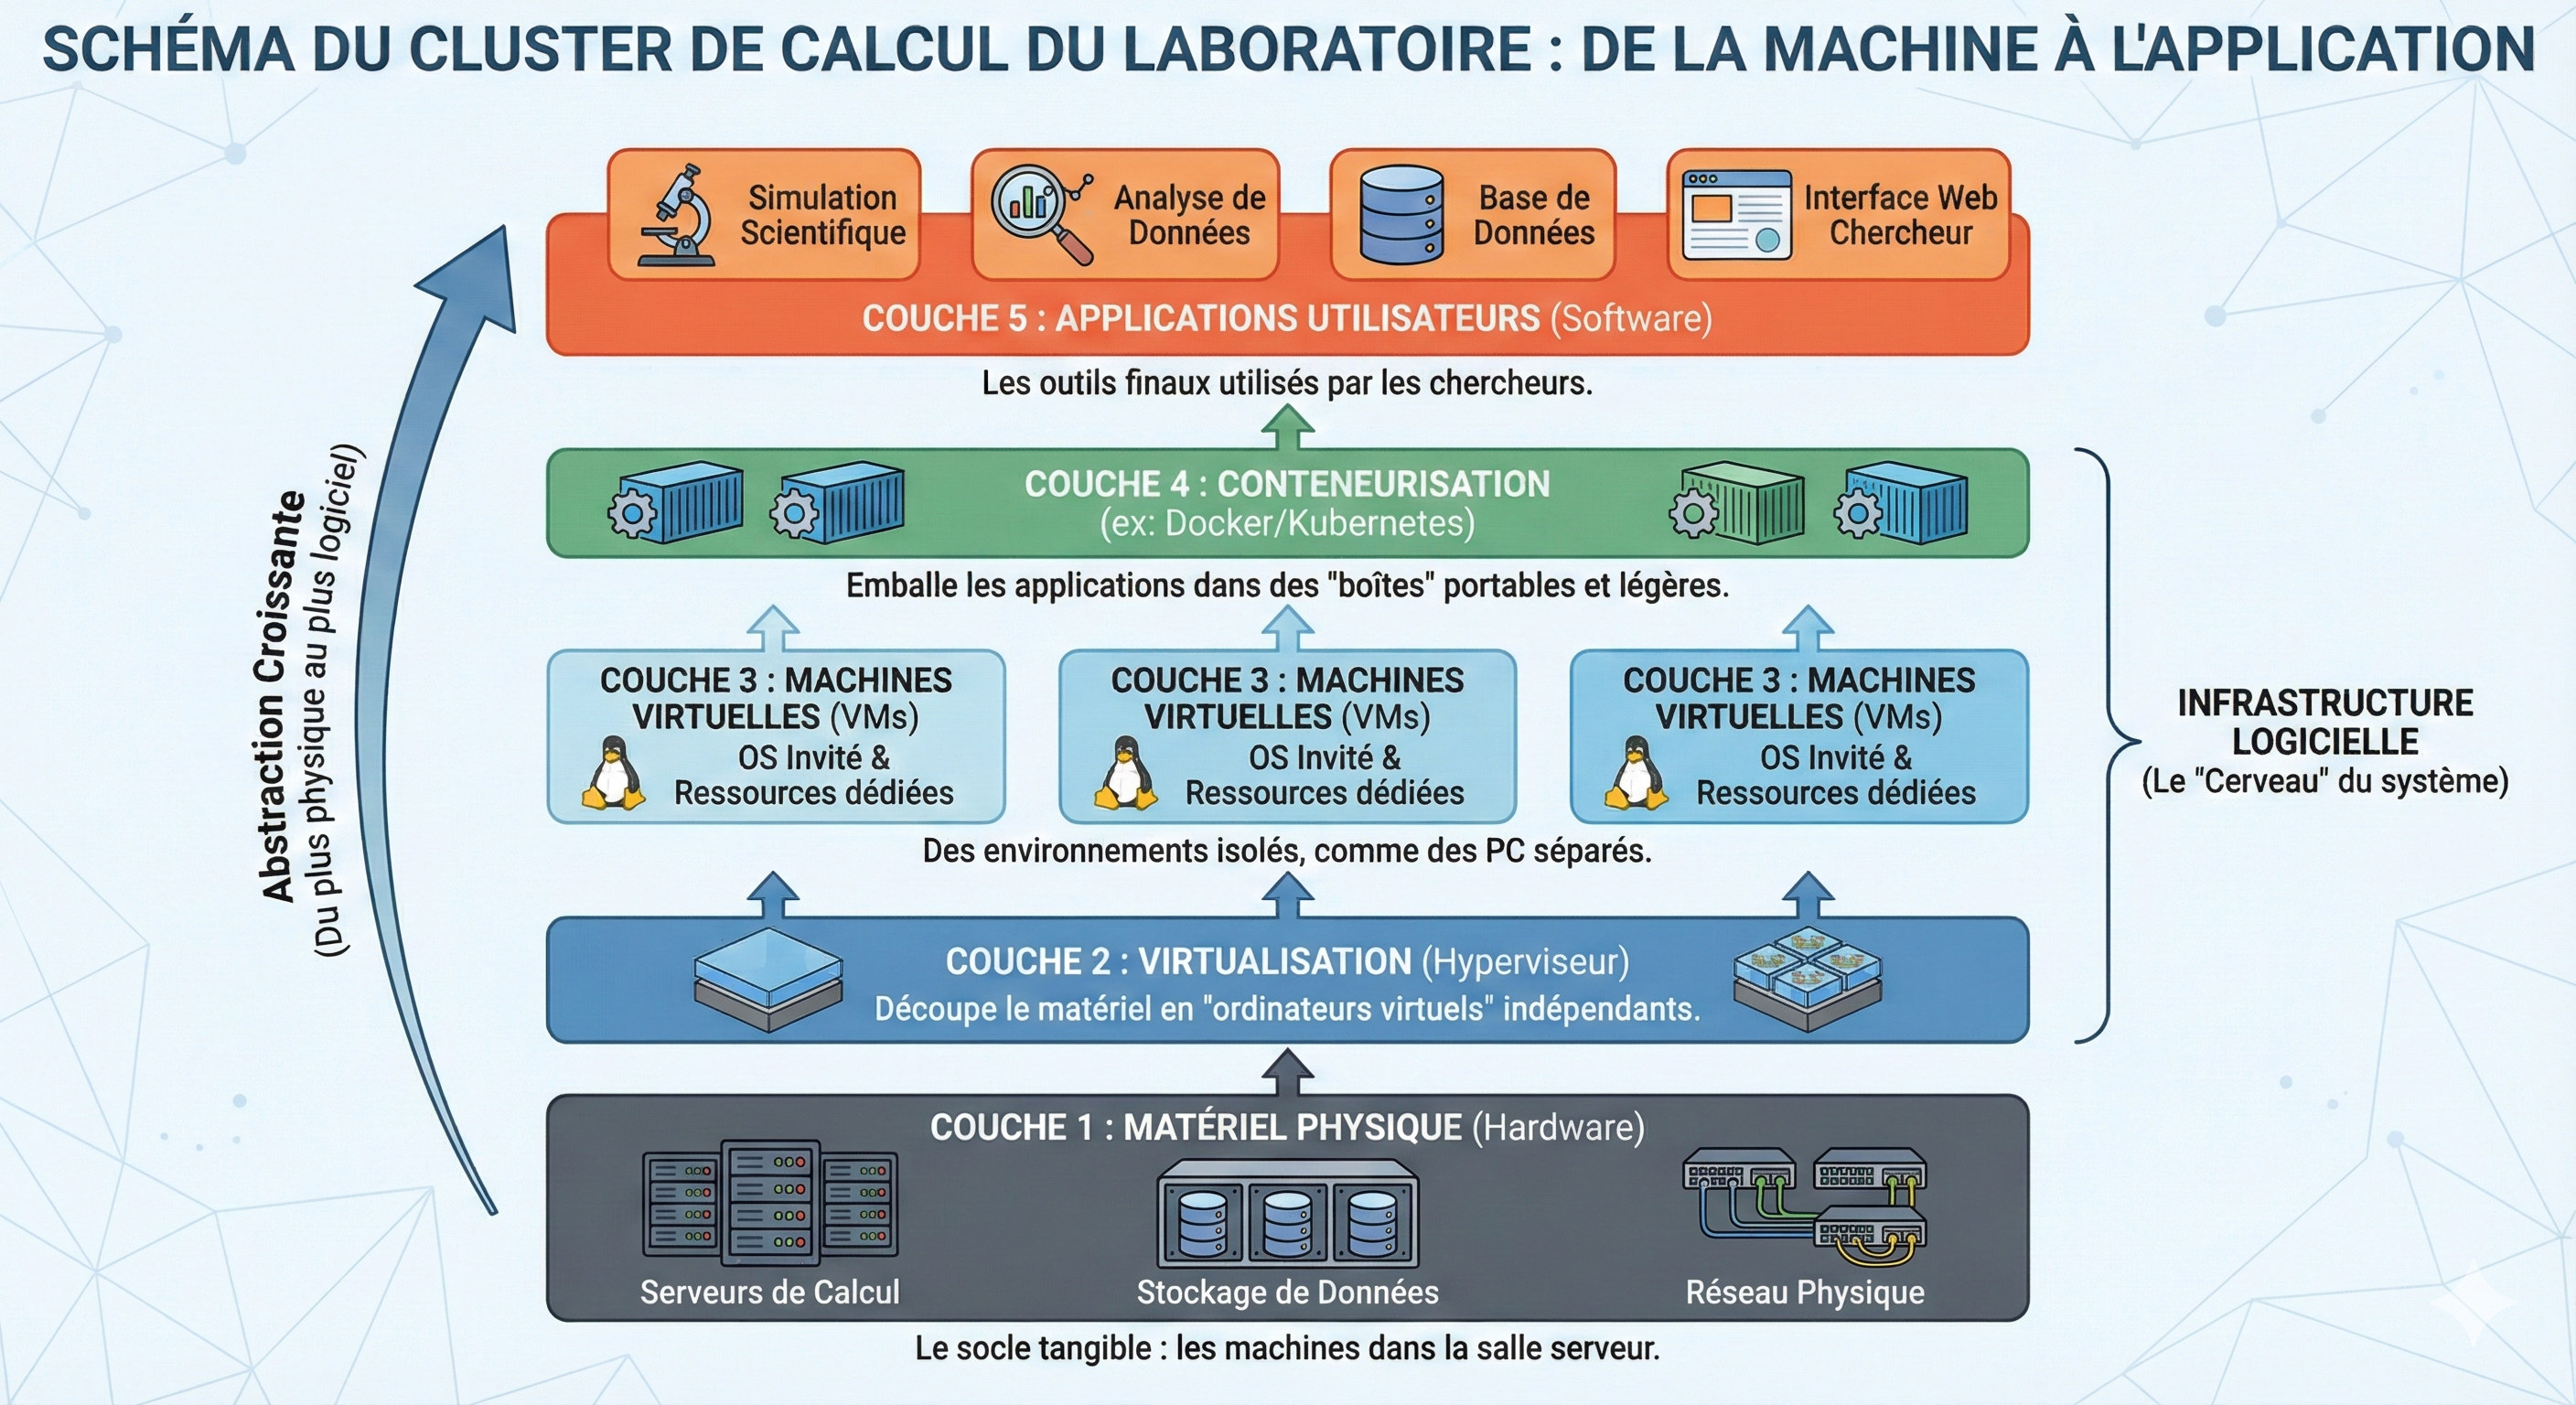
\includegraphics[height=8cm]{img/Gemini_generated_image.png}
    \caption{Exemple de figure avec numérotation continue}
    \label{fig:test_num}
\end{figure}

Comme on le voit sur la \cref{fig:test_num}, le numéro est global.

\section{Bibliographie et Références}

Pour que la bibliographie apparaisse, il faut citer des documents. Voici un exemple de citation d'article \cite{einstein} et de livre \cite{knuth}.

\section{Démonstration des Hyperliens}

Les liens sont désormais colorés selon la charte graphique :
\begin{itemize}
    \item Lien URL : \url{https://www.latex-project.org/}
    \item Lien Texte : \href{https://www.ctan.org/}{CTAN (The Comprehensive TeX Archive Network)}
    \item Référence interne : voir le \cref{chap:intro} (ce chapitre).
\end{itemize}

\section{Listes Personnalisées}

Voici les nouveaux symboles par défaut pour les listes à puces :

\begin{itemize}
    \item Niveau 1 (Défaut)
    \begin{itemize}
        \item Niveau 2
        \begin{itemize}
            \item Niveau 3
        \end{itemize}
    \end{itemize}
\end{itemize}